\begin{defn*}{Vector Component}
    Let $\vec{u}$ and $\vec{v} \neq \overrightarrow{0}$ be vectors. The vector component of $\vec{u}$ in the $\vec{v}$ direction, written $ \operatorname{v-comp}_{\vec{v}} \vec{u}$, is the vector in the direction of $\vec{v}$ so that $\vec{u}-\operatorname{v-comp}_{\vec{v}} \vec{u}$ is orthogonal to $\vec{v}$
	\begin{center}
		\usetikzlibrary{patterns, decorations.pathreplacing}
		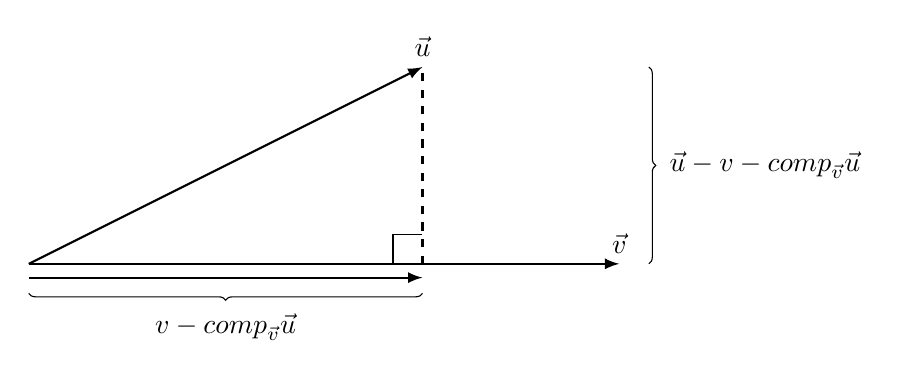
\begin{tikzpicture}[>=latex, scale=2.5]
			\draw[->,thick,black] (0,0) -- (2,1) node [above]
				{$\vec u$};

			\draw[->,thick,black] (0,0) -- (3,0) node [above]
				{$\vec v$};

			\draw[->,thick,black,yshift=-.07cm] (0,0) -- (2,0);
			\draw[decoration={brace, mirror}, decorate, yshift=-.15cm]
                (0,0) -- (2,0) node [midway,below,yshift=-4pt] {$\operatorname{v-comp}_{\vec
				v}\vec u$};

			\draw[dashed,thick,black] (2,0) -- (2,1);
			\draw[decoration={brace, mirror}, decorate, xshift=1.15cm]
				(2,0) -- (2,1) node [midway,right,xshift=4pt]
				{$\vec u-\operatorname{v-comp}_{\vec v}\vec u$};

			\draw[thin,black] (1.85,0)--(1.85,.15)--(2,.15);
		\end{tikzpicture}
	\end{center}
\end{defn*}
